\chapter{Architecture and Design}\label{design}


\section{Data Sources}\label{data_sources}

The vector tiles contain data from multiple data sources. This section describes which data sources where used for which layers in the vector tiles.

\subsection{Custom Curated Labels}

The placement and importance of labels of countries, states and seas matters\cite{12_axismaps.github.io_2015} and is important to get right. Data from the overpass API \cite{13_wiki.openstreetmap.org_2015} is converted into GeoJSON and
manually edited and enhanced with a label rank. For sea labels custom lines have been drawn to place the label along this line.

\begin{table}[H]
\centering
    \begin{tabular}{llll}
    \hline
    Table Name   & Layer Name & Geometry Type & Description \\
    \hline                                          
    custom\_seas       & marine\_label & point    & Marine names \\
    custom\_countries    & country\_label & point    & Country names \\
    custom\_states       & state\_label & point    & State names \\
    \end{tabular}
    \caption{Tables and layers with custom label data}
\end{table}

\subsection{OpenStreetMapData}

Certain \osm{} data like borders and land polygons is very sensitive for change.
The OpenStreetMapData\cite{14_openstreetmapdata.com_2015}
project takes care of a lot of issues that happen with coastlines
and provide it in a convenient format. The data is checked by the OSM community
and released separately.
\\
Water polygons\cite{15_openstreetmapdata.com_2015} from OpenStreetMapData were used for the ocean parts of the world. This data set ensures that the water polygons
work well together with other \osm{} data and splits big water polygons into multiple 
pieces for performance.

\begin{table}[H]
\centering
    \begin{tabular}{llll}
    \hline
    Table Name            & Layer Name & Geometry Type & Description \\
    \hline
    osm\_ocean\_polygon        & water & polygon       & Ocean, seas, large lakes           \\
    osm\_ocean\_polygon\_gen0        & water & polygon       & Simplified ocean, seas, large lakes           \\
    \end{tabular}
    \caption{Table imported from OpenStreetMapData}
\end{table}

\newpage
\subsection{Natural Earth}

The Natural Earth \cite{16_naturalearthdata.com_2015} data set provides manually curated data of cultural and physical features of the world. Natural Earth data is especially useful at higher zoom levels. The imported Natural Earth data results in more than 100 tables, but only a few
are relevant for our use case. The \autoref{data_sources_table} show which Natural Earth tables are used for which layers in the vector tiles.\\\\
The following data sets are used from Natural Earth:

\begin{itemize}
\item Country and administrative borders including disputed borders on lower zoom levels of the admin layer
\item Major lakes and simplified ocean polygons on lower zoom levels of the water layer
\item Label ranks of big cities of the layer place\_label
\end{itemize}

\begin{table}[H]
\centering
    \begin{tabular}{lll}
    \hline
    Table Name                                          & Layer Name & Geometry Type \\
    \hline
    ne\_110m\_admin\_0\_boundary\_lines\_land           & admin & linestring    \\
    ne\_50m\_admin\_0\_boundary\_lines\_land         & admin & linestring    \\
    ne\_50m\_admin\_1\_states\_provinces\_lines            & admin & linestring    \\
    ne\_10m\_admin\_1\_states\_provinces\_lines\_shp            & admin & linestring    \\
    ne\_10m\_admin\_0\_boundary\_lines\_land & admin & linestring    \\
    ne\_10m\_admin\_0\_boundary\_lines\_disputed\_areas & admin & linestring \\
    ne\_110m\_ocean                                       & water & polygon       \\
    ne\_110m\_lakes                                     & water & polygon       \\
    ne\_50m\_ocean                                        & water & polygon       \\
    ne\_50m\_lakes                                      & water & polygon       \\
    ne\_10m\_ocean                                      & water & polygon       \\
    ne\_10m\_lakes                                      & water & polygon       \\
    ne\_10m\_populated\_places                             & place\_label & point       \\
    \end{tabular}
    \caption{Tables imported from Natural Earth}
    \label{data_sources_table}
\end{table}
\clearpage

\section{Architecture}

The architecture of the project is structured into the import phase where the ETL process happens, the changed tile detection phase and the export phase where the vector tiles are rendered. This section describes every component and how it is related to others.

\subsection{Import Components}

The import components take care of importing \osm{} data, external data and SQL views, triggers, indices and functions to help with the rendering and changed tiles detection process.

\subsubsection{Import External}

The \texttt{import-external} component is responsible for importing all data that is not mapped directly from \osm{} into the PostGIS database.

\begin{figure}[H]
  \centering
  \includegraphics[width=1.0\textwidth]{images/import-external-detail-flow-diagram}
  \caption{Barrier layer Schema}
  \label{import_external_diagram} 
\end{figure}

The \autoref{import_external_diagram} shows the external data sources and the bash script which imports it into the database.

\subsubsection{Import OSM}

The \texttt{import-osm} component will take the first PBF file in the ./import folder and will import it into PostGIS. After that it will update the scaleranks using Natural Earth data from \texttt{import-external} to update the scaleranks and will create generalized tables based off the imported data. The data is imported using imposm3 diff mode and can take up to 14hrs for the entire planet file.

\begin{figure}[H]
  \centering
  \includegraphics[width=1.0\textwidth]{images/architecture/import_osm_diagram}
  \caption{Import OSM diagram}
\end{figure}

\subsubsection{Import SQL}

The \texttt{import-sql} component is responsible to import the SQL used for the different layers. It will also generate SQL code for different classifications and code to detect changed tiles and table management commands for different layers.

\begin{figure}[H]
  \centering
  \includegraphics[width=1.0\textwidth]{images/architecture/import_sql_diagram}
  \caption{Import SQL diagram}
\end{figure}

\subsection{Changed Tile Detection Components}

The changed tile detection components handle creating an \osm{} Diff file based on a certain \osm{} planet file, importing a \osm{} Diff file and updating outdated \osm{} planet file with the latest changes. The following sections show what happens in every component.

\subsubsection{Update OSM Diff}

The \texttt{update-osm-diff} component takes the planet file as input and creates an \osm{} Diff file containing all the changes happened since the planet file was downloaded.

\begin{figure}[H]
  \centering
  \includegraphics[width=1.0\textwidth]{images/architecture/update_osm_diff_diagram}
  \caption{Import OSM diagram}
\end{figure}

\subsubsection{Import OSM Diff}

The \texttt{import-osm-diff} component takes the \osm{} Diff file created with the \texttt{update-osm-diff} component as input and imports all changes into the database.

\begin{figure}[H]
  \centering
  \includegraphics[width=1.0\textwidth]{images/architecture/import_osm_diff_diagram}
  \caption{Import OSM diagram}
\end{figure}

\subsubsection{Merge OSM Diff}

The \texttt{merge-osm-diff} component takes the old planet file and the latest diff file as input and merges all changes into the old planet file. Additionally the timestamp of the planet file gets updated in order to get a correct diff file when the \texttt{update-osm-diff} process runs the next time.

\begin{figure}[H]
  \centering
  \includegraphics[width=1.0\textwidth]{images/architecture/merge_osm_diff_diagram}
  \caption{Import OSM diagram}
\end{figure}

\subsubsection{Changed Tiles}

The \texttt{changed-tiles} component is responsible for executing the changed tiles SQL logic and store the list of changed tiles in a text file using pgclimb. The actual logic for detecting the changed tiles is in the \texttt{import-sql} component.

\begin{figure}[H]
  \centering
  \includegraphics[width=1.0\textwidth]{images/architecture/changed_tiles_diagram}
  \caption{Changed Tiles diagram}
\end{figure}

\subsection{Distributed Tile Rendering Components}

In order to meet the performance requirements a distributed rendering architecture 
is needed to scale the process on to multiple hosts and process. The central component of the rendering pipeline is the message queue which contains the rendering jobs and results all other components interact with the message queue to take or confirm a job.

\subsubsection{Generate Jobs}

The \texttt{generate-jobs} component is responsible creating JSON jobs consumed by the \texttt{export} component. It supports two types of jobs:

\begin{itemize}
  \item \textbf{Pyramid}: Job of rendering a tile pyramid (e.g. from z8 all down to z14). Used for initial rendering of the world.
  \item \textbf{List}: Batch jobs of list of tiles to be rendered grouped by data locality. Used for rendering changed tiles.
\end{itemize}

Generate-jobs will output the jobs as individual JSON objects to stdout. A tool like \texttt{pipecat} can be used to schedule them on your job server.

\begin{figure}[H]
  \centering
  \includegraphics[width=1.0\textwidth]{images/architecture/generate_jobs_diagram}
  \caption{Generate Jobs diagram}
\end{figure}
\clearpage

\subsubsection{Export}

The \texttt{export} component is responsible for rendering vector tiles using osm2vectortiles.tm2source and the \texttt{postgis} component. Exports can be run together with a message queue like RabbitMQ or standalone for smaller extracts where it is not necessary to divide the work into several parts.

\begin{figure}[H]
  \centering
  \includegraphics[width=1.0\textwidth]{images/architecture/export_worker_diagram}
  \caption{Export Worker diagram}
\end{figure}

\subsubsection{Merge Jobs}

The \texttt{merge-jobs} component is responsible for taking result messages from the queue, download the attached MBTiles file and merge it into the latest planet MBTiles file.

\begin{figure}[H]
  \centering
  \includegraphics[width=1.0\textwidth]{images/architecture/merge_jobs_flow_diagram}
  \caption{Merge Jobs diagram}
\end{figure}

%------------------------------------------------------
\newpage
\section{Database and Layer Schema}\label{database-schema}

The database schema is denormalized and has no relations. It is heavily optimized for fast reads and the primary and only use case of generating vector tiles from the PostGIS database.

%------------------------------------------------------
\subsection{Aeroways and Airports}

\noindent\begin{minipage}[t]{0.48\linewidth}
    \vspace{0pt}
    The layer \textbf{aeroway} contains infrastructure regarding air travel. The most common features are airports and their aprons, runways and taxiways. Since airports are big landmarks and all features are already present after zoom level 10. The layer consists of polgyons and linestrings (e.g. while runways are often polygons, taxiways are mostly linestrings).
    The layer \textbf{airport\_label} contains labels (either points or centroid of polygons) of airports from airports since airports are important orientation points.
    The \textbf{scalerank} field describes the importance of the airport based on the area and type of the airport.
    The \textbf{ref} field can either be the IATA, FAA, ICAO or other reference code for the airport.
\end{minipage}
\hfill
\begin{minipage}[t]{0.48\linewidth}
    \vspace{-20pt}
    \begin{figure}[H]
      \centering
      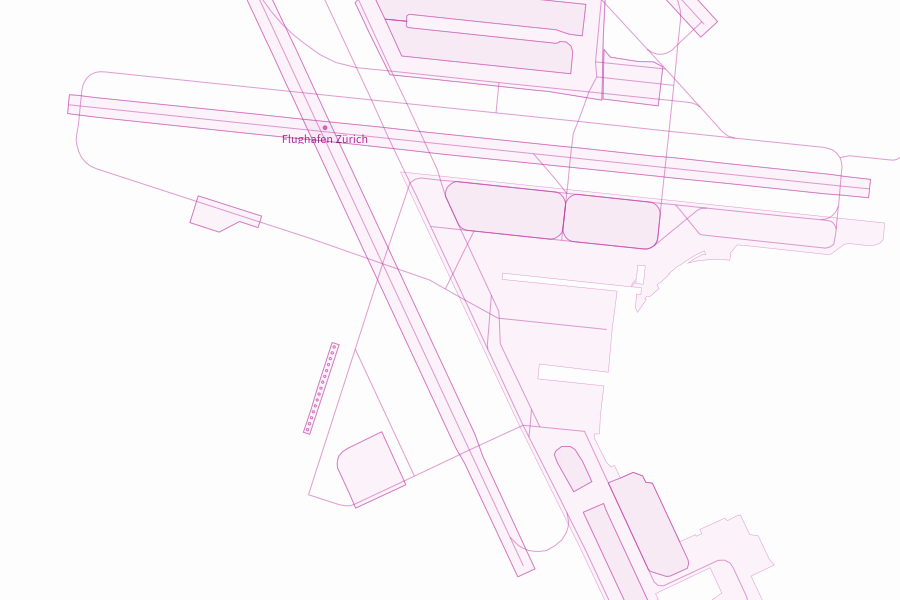
\includegraphics[width=1\textwidth]{images/schema/aeroway_example}
      \caption{Aerowaya and airport label layer of Zurich airport}
    \end{figure}
\end{minipage}

\begin{figure}[H]
  \centering
  \includegraphics[width=0.8\textwidth]{images/schema/aeroway}
  \caption{Aeroway layer}
\end{figure}

\begin{figure}[H]
  \centering
  \includegraphics[width=0.8\textwidth]{images/schema/airport}
  \caption{Airport label layer}
\end{figure}

%------------------------------------------------------
\subsection{Barriers}

\noindent\begin{minipage}[t]{0.48\linewidth}
    \vspace{0pt}
    The layer \textbf{barrier\_line} contains barriers that block a way or path. Common features are structural walls, fences or access controls like bicycle barriers and gates. Man made objects like piers or natural barriers like a cliff are contained as well in the \textbf{barrier\_line} layer. Despite the layer name barriers can not only be linestrings (e.g. walls) but polygons as well (e.g. piers). Barriers are only relevant at the highest zoom level 14.
\end{minipage}
\hfill
\begin{minipage}[t]{0.48\linewidth}
    \begin{figure}[H]
      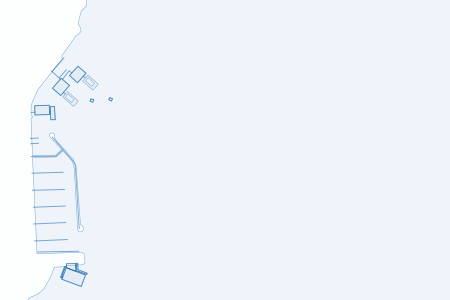
\includegraphics[width=1\textwidth]{images/schema/piers_example}
      \caption{Barrier line layer with piers at Lake Zurich}
    \end{figure}
\end{minipage}

\begin{figure}[H]
  \centering
  \includegraphics[width=0.8\textwidth]{images/schema/barrier_line}
  \caption{Barrier layer Schema}
\end{figure}

%------------------------------------------------------
\subsection{Road and Road Labels}

\noindent\begin{minipage}[t]{0.48\linewidth}
    \vspace{0pt}
    Roads are one of the most essential features in maps. Roads are present across all zoom levels filtered by their importance. The \textbf{road} and \textbf{road\_label} layer query the data from the \textbf{road\_geometry} table where both polygons and linestrings are present.
    
    The \textbf{road\_label} layer consists of linestrings that have a name assigned and are also encoded as linestrings in the vector tile. The client renderer then takes care of putting the road label across the road linestring.
\end{minipage}
\hfill
\begin{minipage}[t]{0.48\linewidth}
    \begin{figure}[H]
      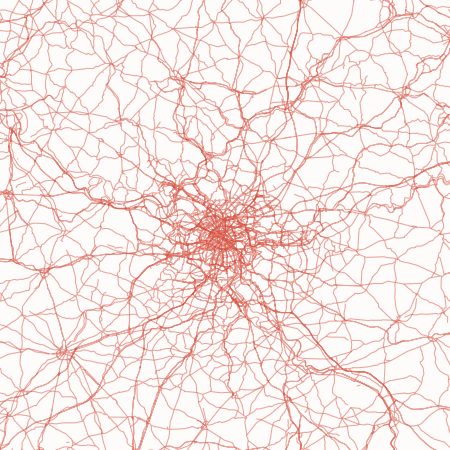
\includegraphics[width=1\textwidth]{images/schema/road_example}
      \caption{Road layer around Paris}
    \end{figure}
\end{minipage}

\begin{figure}[H]
  \centering
  \includegraphics[width=0.8\textwidth]{images/schema/road}
  \caption{Road layer schema}
\end{figure}

%------------------------------------------------------
\subsection{Water}


\noindent\begin{minipage}[t]{0.48\linewidth}
    \vspace{0pt}
    The \textbf{water} layer contains all bodies of water be it ocean, lakes or large rivers.
    Since water is so essential for the quality of the map a variety of different sources is used on different zoom levels. At low zoom levels 0 to 4 already generalized NaturalEarth data is used for both ocean and lake polygons. On zoom level 5 to 14 water data imported from \osm{} and split ocean polygons from OpenStreetMap data are used. Very large water polygons are split due to performance reasons.
    The \textbf{water\_label} layer shows the labels of lake bodies (not marine waters). Those are precalculated from the centroid of the water polygon in the \textbf{water\_point} table.
\end{minipage}
\hfill
\begin{minipage}[t]{0.48\linewidth}
    \vspace{-20pt}
    \begin{figure}[H]
      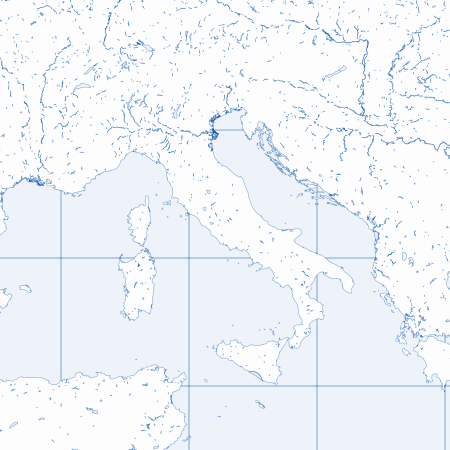
\includegraphics[width=1\textwidth]{images/schema/water_example}
      \caption{Tiled ocean and water bodies in Europe at zoom level 5}
    \end{figure}
\end{minipage}

\begin{figure}[H]
  \centering
  \includegraphics[width=0.8\textwidth]{images/schema/water}
  \caption{Water layer schema}
\end{figure}

%------------------------------------------------------
\subsection{Buildings and Housenumbers}

\noindent\begin{minipage}[t]{0.48\linewidth}
    \vspace{0pt}
    Building are polygons for a building structure such as a house. Buildings only appear on the highest zoom level 14 with the exceptions of very large buildings already appearing at zoom level 13.
    Some buildings are also tagged with a housenumber (the housenumber might also be a single point in OSM). These housenumber labels are rendered in the \textbf{housenum\_label} layer. Housenumber only appear at zoom level 14.
\end{minipage}
\hfill
\begin{minipage}[t]{0.48\linewidth}
    \vspace{-20pt}
    \begin{figure}[H]
      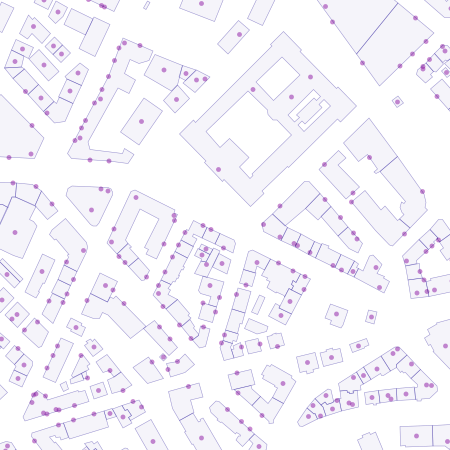
\includegraphics[width=1\textwidth]{images/schema/building_example}
      \caption{Buildings and house numbers}
    \end{figure}
\end{minipage}

\begin{figure}[H]
  \centering
  \includegraphics[width=0.8\textwidth]{images/schema/building}
  \caption{Building layer schema}
\end{figure}

%------------------------------------------------------
\subsection{Administrative Borders}

\noindent\begin{minipage}[t]{0.48\linewidth}
    \vspace{0pt}
    The \textbf{admin} layer contains the linestrings of administrative boundaries such as countries, states or provinces. Since a different level of detail is required at different zoom levels NaturalEarth data is used at very low zoom levels for countries and very large provinces while at higher zoom levels the more accurate \osm{} data is used. Boundaries are treated as linestrings because borders often break in \osm{} and can then no longer be reconstructed as polygons. Therefore it is safer to work with them as linestrings even thought this provides less options for e.g. coloring different administrative areas.
\end{minipage}
\hfill
\begin{minipage}[t]{0.48\linewidth}
    \vspace{-20pt}
    \begin{figure}[H]
      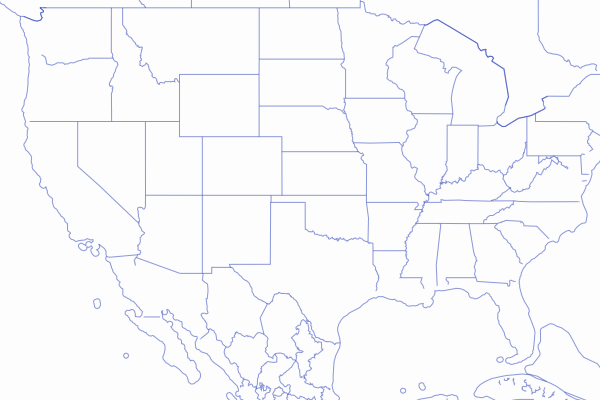
\includegraphics[width=1\textwidth]{images/schema/admin_example}
      \caption{Admin level 4 (states) in the US}
    \end{figure}
\end{minipage}

\vspace{20}

\begin{figure}[H]
  \centering
  \includegraphics[width=1\textwidth]{images/schema/admin}
  \caption{Admin layer schema}
\end{figure}

%------------------------------------------------------
\subsection{Landuse and Landuse Overlay}

\noindent\begin{minipage}[t]{0.48\linewidth}
    \vspace{0pt}
    The layer \textbf{landuse} of contains polygons of specially zoned land. The most frequent 
    features inside \textbf{landuse} are wood areas as well as national parks, swamps, commercial, industrial and military zones.
    Very large polygons are split into several pieces into the \textbf{landuse\_split\_polygon} table and large polygons are generalized
    for lower zoom levels. The Polygons on the \textbf{landuse} layer are filtered by their covered area depending on the zoom level with only
    the largest polygons being shown at low zoom levels.
\end{minipage}
\hfill
\begin{minipage}[t]{0.48\linewidth}
    \vspace{-20pt}
    \begin{figure}[H]
      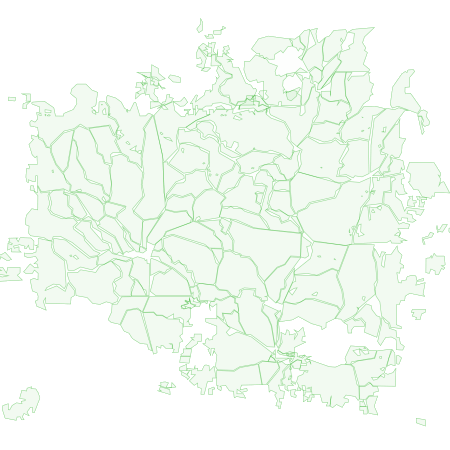
\includegraphics[width=1\textwidth]{images/schema/landuse_example}
      \caption{Landuse (wood) at zoom level 10}
    \end{figure}
\end{minipage}

\begin{figure}[H]
  \centering
  \includegraphics[width=0.8\textwidth]{images/schema/landuse}
  \caption{Landuse layer schema}
\end{figure}

%------------------------------------------------------
\subsection{POI Labels}

\noindent\begin{minipage}[t]{0.48\linewidth}
    \vspace{0pt}
    A point of interest (POI) is a feature bound to a particular point of the map (e.g. churches, schools, tourist attractions, hotels, trees).
    Not all POIs are relevant and to appear on the map, POIs are required to have at least a name or icon derived from the \textbf{type} field.
    Since users shouldn't be overwhelmed with information on a map the field \textbf{localrank} contains an ascending importance rank which can be used by map clients to show important POIs first and very prominent POIs also have a scalerank based on their covered \textbf{area}. The rank calculation for POIs works very similar to place label ranking described in \autoref{place_label_rank_calc}.
\end{minipage}
\hfill
\begin{minipage}[t]{0.48\linewidth}
    \vspace{0pt}
    \begin{figure}[H]
        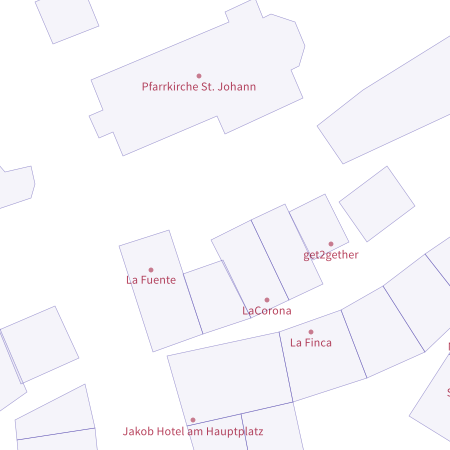
\includegraphics[width=\textwidth]{images/schema/poi_label_example}
        \caption{POI layer on top of building layer}
    \end{figure}
\end{minipage}
\vspace{20pt}
\begin{figure}[h]
  \centering
  \includegraphics[width=0.8\textwidth]{images/schema/poi_label}
  \caption{POI label layer schema}
\end{figure}

%---------------------------------
\subsection{Country and State Labels}

\noindent\begin{minipage}[t]{0.48\linewidth}
    \vspace{0pt}
    Names and placement of country and state labels are very important.
    Because it is difficult to ensure quality of these features when importing directly from \osm{} the countries and states are pulled from \osm{} data once
    and get the \textbf{scalerank} assigned by hand to ensure label
    importance ranking and label placement are as good as possible.
    This effort is worth it because country and state data changes
    at infrequent intervals.
    Country labels are not present on all zoom levels and are filtered based
    on their \textbf{scalerank} value to show countries like Italy prior to a less important city state like the Vatican.
\end{minipage}
\hfill
\begin{minipage}[t]{0.48\linewidth}
    \vspace{0pt}
    \begin{figure}[H]
        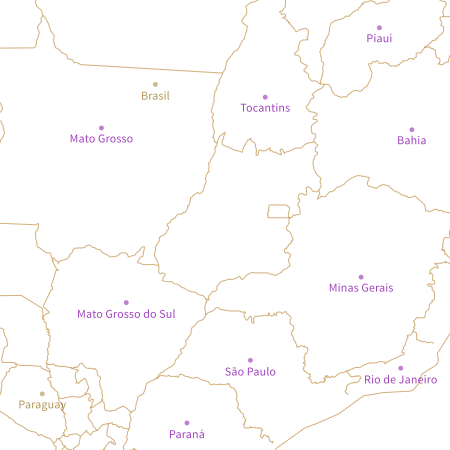
\includegraphics[width=\textwidth]{images/schema/country_state_label_example}
        \caption{Country and state labels around Brasil}
    \end{figure}
\end{minipage}

\begin{figure}[H]
  \centering
  \includegraphics[width=0.8\textwidth]{images/schema/country_state}
  \caption{Country and state layer schema}
\end{figure}

%------------------------------------------------------
\subsection{Place Labels}

\noindent\begin{minipage}[t]{0.48\linewidth}
    \vspace{0pt}
    Place labels help for intermediate orientation. It is important to show only
    world cities at low zoom levels and then gradually show more and more local places. Filtering happens over the \textbf{scalerank} and \textbf{localrank}
    fields in the vector tiles. Since place labels are very delicate and important
    every zoom level has custom filters for which places are relevant.
    The rank calculation for places is explained in \autoref{place_label_rank_calc}.
\end{minipage}
\hfill
\begin{minipage}[t]{0.48\linewidth}
    \vspace{-20pt}
    \begin{figure}[H]
      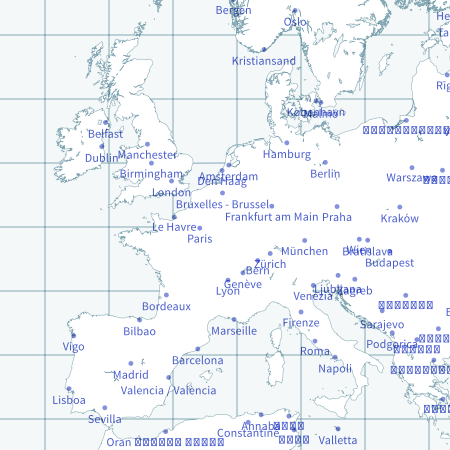
\includegraphics[width=1\textwidth]{images/schema/place_example}
      \caption{Important place labels in Europe}
    \end{figure}
\end{minipage}

\begin{figure}[H]
  \centering
  \includegraphics[width=1\textwidth]{images/schema/place_label}
  \caption{Place label layer }
\end{figure}
